\documentclass{article}

\usepackage{graphicx}
%\usepackage{fullpage}
\usepackage{fancyhdr}
\pagestyle{fancy}
\renewcommand{\headrulewidth}{0pt}
\lhead{}
\rhead{}

\usepackage[printwatermark]{xwatermark}
\usepackage{xcolor}

%\textheight=9.0in

%\pagestyle{empty}
%\raggedbottom
%\raggedright

\pagenumbering{arabic}

\title{Ka Downlink}
\author{Tate Walker}

\begin{document}

\maketitle

Link Budget Report for PPE Module of Gateway

\newpage
\section{Orbit}
\label{section::orbit}
\begin{center}
  \begin{tabular}{p{3in}p{1in}l}
\textbf{Orbit} & & \\
\hline \\
Apoapsis & 426452 & $km$ \\
Periapsis & 356873 & $km$ \\
Mean Altitude & 391662.50 & $km$ \\
\\
\textbf{Constants} & & \\
\hline \\
Earth Radius & 6378.14 & $km$ \\
GS Angle of Elevation & 20 & $^{\circ}$ \\
\\
\textbf{Key Outputs} & & \\
\hline \\
Slant Range & 395814.06 & $km$ \\
Satellite Angle from Boresight & 0.86 & $^{\circ}$ \\
\\
\end{tabular}

\end{center}

\newpage
\section{Transmitter}
\label{section::transmitter}
\begin{center}
  \begin{tabular}{p{3in}p{1in}l}
\textbf{Antenna} & & \\
\hline \\
Sampled Gain & 3.00 & $dBi$ \\
Antenna Pointing Loss & 0 & $dB$ \\
Gain at Boresight & 3.00 & $dBi$ \\
Average Nadir Gain & -0.18 & $dBi$ \\
Polarization & RHCP & $$ \\
\\
\textbf{Transmitter (Satellite Ka-Band Transmitter)} & & \\
\hline \\
Transmit Power at PA & 50 & $dBW$ \\
Inline Losses & 0 & $dB$ \\
Transmit Power at Antenna & 50 & $dBW$ \\
EIRP & 53.00 & $dBW$ \\
\\
\end{tabular}

  \begin{figure}
    \caption{TX Antenna Gain Pattern}
    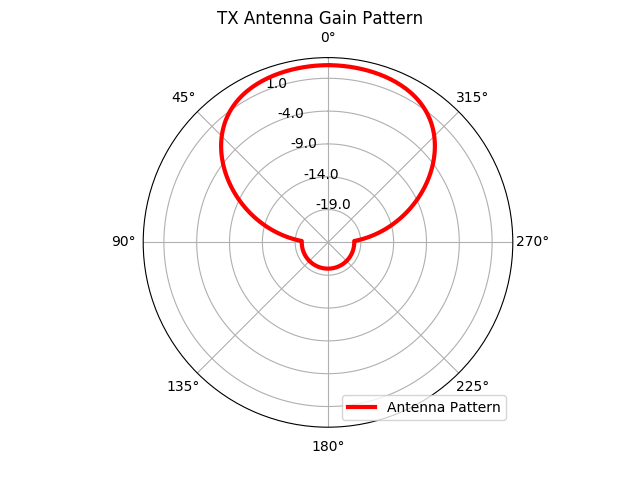
\includegraphics[width=\linewidth]{Ka_DownlinkTXPattern.png}
    \label{fig::pattern::tx}
  \end{figure}
\end{center}


\newpage
\section{Channel}
\label{section::channel}
\begin{center}
  \begin{tabular}{p{3in}p{1in}l}
\textbf{Constants} & & \\
\hline \\
Center Frequency & 26.00 & $GHz$ \\
Speed of Light & 299792458 & $m/s$ \\
Allocated Bandwidth & 5.00 & $MHz$ \\
Start of Allocation & 26.00 & $GHz$ \\
End of Allocation & 26.00 & $GHz$ \\
Wavelength & 1.15 & $cm$ \\
\\
\textbf{Losses} & & \\
\hline \\
Unity Gain Propagation Loss & 232.70 & $dB$ \\
Atmospheric Loss & 1 & $dB$ \\
Ionospheric Loss & 1 & $dB$ \\
Rain Loss & 2 & $dB$ \\
Multipath Fading Loss & 0 & $dB$ \\
Total Channel Loss & 236.70 & $dB$ \\
\\
\textbf{Modulation (DVB-S2X)} & & \\
\hline \\
Modulation Name & DVB-S2X & $$ \\
Modulation Code & QPSK 13/45 & $$ \\
Tx Spectral Efficiency & 0.45 & $$ \\
Bitrate & 1.00 & $MHz$ \\
Bitrate & 60.00 & $dBHz$ \\
Required Demodulation $E_b/N_0$ & 0.43 & $dB$ \\
Required Demod Bandwidth & 1.76 & $MHz$ \\
Required Demod Bandwidth & 62.46 & $dBHz$ \\
Required Transmit Bandwidth & 63.43 & $dBHz$ \\
\\
\end{tabular}

\end{center}


\newpage
\section{Receiver}
\label{section::receiver}
\begin{center}
  \begin{tabular}{p{3in}p{1in}l}
\textbf{Antenna} & & \\
\hline \\
Noise Temperature & 300 & $K$ \\
Sampled Gain & 48.00 & $dBi$ \\
Antenna Pointing Loss & 0 & $dB$ \\
Gain at Boresight & 48.00 & $dBi$ \\
Average Nadir Gain & -8.78 & $dBi$ \\
Polarization & LCP & $$ \\
\\
\textbf{System} & & \\
\hline \\
Total Receiver Noise Temperature & 666.84 & $K$ \\
Total Receiver Noise Temperature & 28.24 & $dBK$ \\
Receive Chain Noise Temperature & 366.84 & $K$ \\
Receive Chain Noise Factor & 2.26 & $$ \\
Receive Chain Noise Figure & 3.55 & $dB$ \\
Receiver Noise Bandwidth & 1.00 & $MHz$ \\
Implementation Loss & 0 & $dB$ \\
\\
\end{tabular}

  \vspace{0.1in}
  \hspace*{-0.75in} \begin{tabular}{p{1.25in}p{0.47in}p{0.47in}p{0.5in}p{0.6in}p{0.5in}p{0.5in}p{0.75in}}
\textbf{Element} & \textbf{Gain} & \textbf{Noise Figure} & \textbf{Noise Temp.} & \textbf{Upstream Gain Factor} & \textbf{Contrib. Noise Temp} & \textbf{Contrib. Noise Factor} & \textbf{Noise Temp Pct Contrib.}\\
\hline \\
 & \textbf{$dB$} & \textbf{$dB$} & \textbf{$K$} &  & \textbf{$K$} &  & \textbf{$\%$}\\
\hline \\
Cables & -0.75 & 0.75 & 54.67 & 1 & 54.67 & 0.19 & 14.90\\
LNA & 35.00 & 2.75 & 256 & 0.84 & 304 & 1.05 & 83.02\\
Filter & -3.50 & 3.50 & 359 & 2660 & 0.14 & 0.00 & 0.04\\
Demodulator & 0.00 & 15.00 & 8880 & 1188 & 7.47 & 0.03 & 2.04\\
\end{tabular}
  \begin{figure}
    \caption{RX Antenna Gain Pattern}
    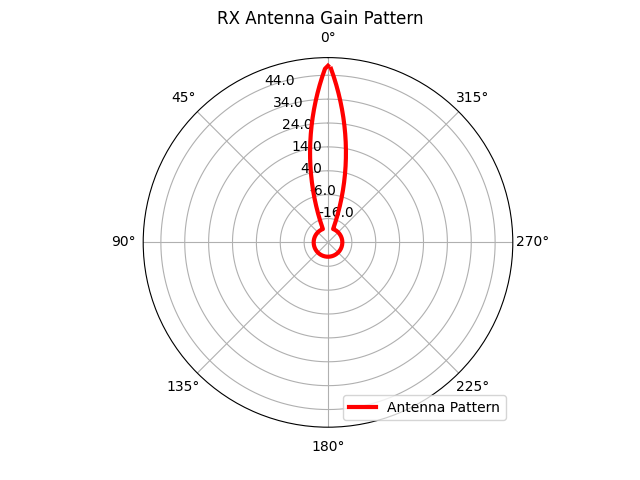
\includegraphics[width=\linewidth]{Ka_DownlinkRXPattern.png}
    \label{fig::pattern::rx}
  \end{figure}
\end{center}


\newpage
\section{Interference}
\label{section::interference}
\begin{center}
  \begin{tabular}{p{3in}p{1in}l}
\textbf{Transmitter (Satellite Ka-Band Transmitter)} & & \\
\hline \\
Transmit Power at Antenna & 50 & $dBW$ \\
Peak Antenna Gain & 3.00 & $dBi$ \\
Peak EIRP & 53.00 & $dBW$ \\
Nadir-to-GS Gain & 3.00 & $dBi$ \\
Nadir-to-GS EIRP & 53.00 & $dBW$ \\
Average Antenna Gain & -12.15 & $dBi$ \\
\\
\textbf{Peak Power Flux Density at Receiver} & & \\
\hline \\
Peak PFD at Surface per 1kHz & -161.50 & $dBW/m^2/1kHz$ \\
Peak PFD at Surface per 4kHz & -155.48 & $dBW/m^2/4kHz$ \\
Peak PFD at Surface per 1MHz & -131.50 & $dBW/m^2/1MHz$ \\
Peak PFD at GSO per 1kHz & -162.29 & $dBW/m^2/1kHz$ \\
Peak PFD at GSO per 4kHz & -156.27 & $dBW/m^2/4kHz$ \\
Peak PFD at GSO per 1MHz & -132.29 & $dBW/m^2/1MHz$ \\
\\
\textbf{Hey Regulators, Look In this Section} & & \\
\hline \\
Lowest Permissible PFD (4kHz BW) at Receiver & -150 & $dBW/m^2$ \\
Peak Possible PFD (4kHz BW) at Receiver & -160.01 & $dBW/m^2$ \\
\\
\end{tabular}

  
\end{center}


\newpage
\section{Bitrates (Custom Section Example)}
\label{section::Bitrates_(Custom_Section_Example)}
\begin{center}

\begin{tabular}{p{3in}p{1in}l}
\textbf{Bitrate Requirements for TT\&C} & & \\
\hline \\
Number of Log Files & 1000 & $$ \\
Size of Each Log File & 16 & $kB$ \\
Minimum Average Bitrate & 9600 & $kbps$ \\
\\
\textbf{Bitrate Requirements for Images} & & \\
\hline \\
Number of Images & 1000 & $$ \\
Size of Each Image & 32 & $MB$ \\
Minimum Average Bitrate & 32 & $mbps$ \\
\\
\end{tabular}

\end{center}

\newpage
\section{Budget}
\label{section::budget}
\begin{center}
  \begin{tabular}{p{3in}p{1in}l}
\textbf{Transmitter (Satellite Ka-Band Transmitter)} & & \\
\hline \\
Power at Antenna & 50 & $dBW$ \\
Gain & 3.00 & $dBi$ \\
Antenna Pointing Loss & 0 & $dB$ \\
EIRP & 53.00 & $dBW$ \\
\\
\textbf{Channel} & & \\
\hline \\
Center Frequency & 26.00 & $GHz$ \\
Free Space Loss & 232.70 & $dB$ \\
Total Channel Loss & 236.70 & $dB$ \\
Occupied Bandwidth & 63.43 & $dBHz$ \\
\\
\textbf{Receiver (Ground Ka-Band Receiver)} & & \\
\hline \\
Signal Power Flux at RX Antenna & -133.94 & $dBW/m^2$ \\
Antenna Gain & 48.00 & $dBi$ \\
Antenna Effective Area & -1.76 & $dBm^2$ \\
Polarization Mismatch Loss & 3 & $dB$ \\
RX System Noise Temperature & 666.84 & $K$ \\
RX Figure of Merit ($G/T$) & 19.76 & $dB/K$ \\
Noise Spectral Density ($N_0$) & -200.36 & $dBW/Hz$ \\
Received Signal Power & -138.70 & $dBW$ \\
Excess Noise BW Loss & 0.00 & $dB$ \\
Implementation Loss & 0 & $dB$ \\
Required Demodulation $E_b/N_0$ & 0.43 & $dB$ \\
Antenna Pointing Loss & 0 & $dB$ \\
Carrier to Noise ($C/N_0$) & 61.66 & $dBHz$ \\
\\
\textbf{Eb/N0} & & \\
\hline \\
BitRate & 60.00 & $dBHz$ \\
Energy per Bit ($E_b$) & -198.70 & $dBW/Hz$ \\
Received $E_b/N_0$ & 1.66 & $dB$ \\
Required $E_b/N_0$ & 0.43 & $dB$ \\
\\
\textbf{Key Outputs} & & \\
\hline \\
Bitrate & 1.00 & $MHz$ \\
Link Margin & 1.23 & $dB$ \\
\\
\end{tabular}

  
  \begin{figure}
    \caption{Bitrate with 1dB of Link Margin vs Elevation}
    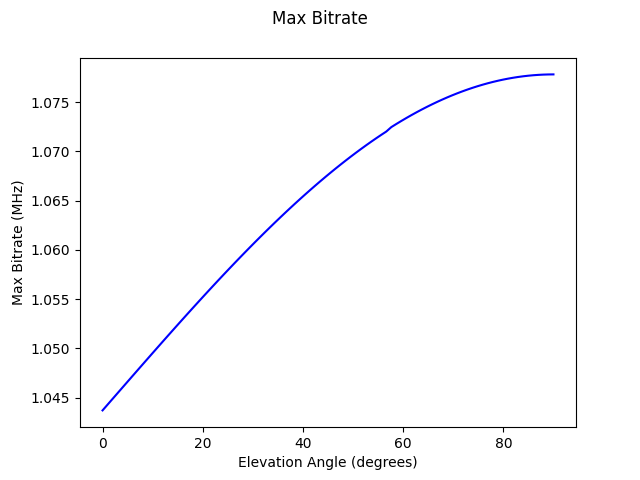
\includegraphics[width=\linewidth]{./max-bitrate.png}
    \label{fig::pfd::max-bitrate}
  \end{figure}
        
\end{center}

\newpage
So long, and thanks for all the Fish!

\lfoot{Brought to you by \href{http://github.com/harrison-caudill/pylink}{PyLink}}

\end{document}